\documentclass[10pt]{scrartcl}
\usepackage[mdthm,colorsec,noauthor,noasy]{evan}
\usepackage{handout}
\usepackage[T1]{fontenc}
\usepackage{lmodern}
\usepackage{listings}
\lstset{language=Python,emptylines=1,basicstyle=\ttfamily\normalsize,identifierstyle=\color{black},keywordstyle=\color{NavyBlue},commentstyle=\color{black!60},stringstyle=\color{RawSienna},showstringspaces=false,columns=fullflexible,keepspaces=true,upquote=true,aboveskip=5pt,belowskip=5pt}
\newcommand{\py}[1]{\texttt{#1}}
\newcommand{\hint}[1]{\par\emph{Hint:} #1\par}
\newcommand{\codeblock}[1]{\par\noindent\begin{minipage}{\linewidth}\csname code#1\endcsname\end{minipage}\par}
\expandafter\def\csname codeswipe\endcsname{\lstinputlisting[firstline=4,lastline=10]{discussion_solutions.py}}
\expandafter\def\csname codeskip_fact\endcsname{\lstinputlisting[firstline=14,lastline=17]{discussion_solutions.py}}
\expandafter\def\csname coderecursive_prime\endcsname{\lstinputlisting[firstline=21,lastline=29]{discussion_solutions.py}}
\expandafter\def\csname codehailstone\endcsname{\lstinputlisting[firstline=33,lastline=45]{discussion_solutions.py}}
\expandafter\def\csname codesevens\endcsname{\lstinputlisting[firstline=49,lastline=68]{discussion_solutions.py}}
\expandafter\def\csname codekarel\endcsname{\lstinputlisting[firstline=72,lastline=84]{discussion_solutions.py}}
\expandafter\def\csname codeall_digits\endcsname{\lstinputlisting[firstline=4,lastline=9]{exam_solutions.py}}
\expandafter\def\csname codeprefix_process\endcsname{\lstinputlisting[firstline=13,lastline=21]{exam_solutions.py}}
\expandafter\def\csname codeprefix_loop\endcsname{\lstinputlisting[firstline=25,lastline=33]{exam_solutions.py}}
\expandafter\def\csname codenumbered_hailstone\endcsname{\lstinputlisting[firstline=37,lastline=47]{exam_solutions.py}}
\expandafter\def\csname codecollapse\endcsname{\lstinputlisting[firstline=51,lastline=58]{exam_solutions.py}}
\expandafter\def\csname codecontains\endcsname{\lstinputlisting[firstline=62,lastline=70]{exam_solutions.py}}
\expandafter\def\csname codereverse_curry\endcsname{\lstinputlisting[firstline=4,lastline=15]{examples.py}}
\expandafter\def\csname codeexp_parent\endcsname{\lstinputlisting[firstline=19,lastline=22]{examples.py}}
\expandafter\def\csname codesum_digits\endcsname{\lstinputlisting[firstline=26,lastline=30]{examples.py}}
\expandafter\def\csname codefact\endcsname{\lstinputlisting[firstline=34,lastline=37]{examples.py}}
\expandafter\def\csname codefact_iter\endcsname{\lstinputlisting[firstline=41,lastline=45]{examples.py}}
\expandafter\def\csname codefact_k\endcsname{\lstinputlisting[firstline=49,lastline=59]{examples.py}}
\expandafter\def\csname codeplay\endcsname{\lstinputlisting[firstline=63,lastline=72]{examples.py}}
\expandafter\def\csname codeparity\endcsname{\lstinputlisting[firstline=76,lastline=84]{examples.py}}
\expandafter\def\csname codecascade\endcsname{\lstinputlisting[firstline=88,lastline=92]{examples.py}}
\expandafter\def\csname codealice_bob\endcsname{\lstinputlisting[firstline=96,lastline=108]{examples.py}}
\expandafter\def\csname codeunique_factors\endcsname{\lstinputlisting[firstline=112,lastline=127]{examples.py}}
\expandafter\def\csname codefib\endcsname{\lstinputlisting[firstline=131,lastline=136]{examples.py}}
\expandafter\def\csname codepartitions\endcsname{\lstinputlisting[firstline=140,lastline=147]{examples.py}}
\expandafter\def\csname codeparking\endcsname{\lstinputlisting[firstline=151,lastline=156]{examples.py}}
\expandafter\def\csname codestreak\endcsname{\lstinputlisting[firstline=160,lastline=162]{examples.py}}
\expandafter\def\csname codenum_eights\endcsname{\lstinputlisting[firstline=4,lastline=9]{hw_solutions.py}}
\expandafter\def\csname codedistance\endcsname{\lstinputlisting[firstline=13,lastline=16]{hw_solutions.py}}
\expandafter\def\csname codeinterleaved\endcsname{\lstinputlisting[firstline=20,lastline=29]{hw_solutions.py}}
\expandafter\def\csname codecoins\endcsname{\lstinputlisting[firstline=33,lastline=49]{hw_solutions.py}}
\expandafter\def\csname codemax_subseq\endcsname{\lstinputlisting[firstline=53,lastline=58]{hw_solutions.py}}
\expandafter\def\csname codehanoi\endcsname{\lstinputlisting[firstline=62,lastline=73]{hw_solutions.py}}
\expandafter\def\csname codeanonymous\endcsname{\lstinputlisting[firstline=77,lastline=81]{hw_solutions.py}}

\title{CS 61A --- Week 4}
\subtitle{September 14--20: Recursion and Tree Recursion\\Lectures 8--10; Composing Programs 1.7; Discussion 3; HW3}
\author{}\date{}\ihead{}
\begin{document}\maketitle
\section{Choose a smaller instance of the same task}
\begin{qbox}
To sum the digits of 738, what work remains after separating the last digit 8? Why does calling the same function again not overwrite its first input?
\end{qbox}
A function is \textbf{recursive} when its body calls itself directly, or calls another function that eventually calls it. Recursion uses the ordinary call rules: each user-defined call has a separate local frame. Its parent is the function's defining frame, rather than the previous recursive call. An unfinished call waits for the value needed by its return expression.
\begin{proposition*}[Recursive correctness --- CP 1.7; Lecture 10 slide 4]
State the result required for every input. Identify base cases whose results need no recursive call. For any other input, show that the recursive calls solve smaller instances and that their results combine into the specified answer. If each call decreases a nonnegative integer measure until a base case, this also proves termination. Correctly combining results and eventually reaching a base case are separate requirements.
\end{proposition*}
For positive integer $n$, the last digit is \py{n\%10}; the preceding digits form \py{n//10}. A one-digit number is already its own digit sum.
\begin{motive}
\ii[Want.] Compute a digit sum without storing the entire sequence of digits.
\ii[Know.] Removing the last digit leaves exactly the same task on a shorter number.
\ii[Key step.] Ask the recursive call for the preceding digits' sum, then add the one digit that was removed. The original call retains that last digit in its own frame while it waits.
\end{motive}
\codeblock{sum_digits}
\begin{fig}
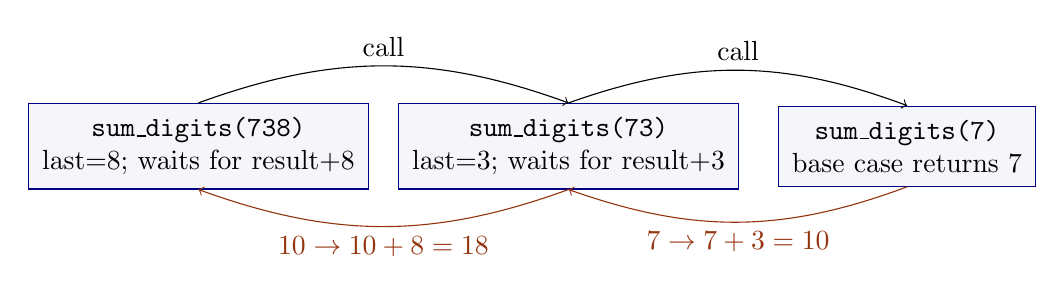
\begin{tikzpicture}[box/.style={draw=NavyBlue,fill=NavyBlue!4,align=center,inner sep=5pt}]
\node[box] (a) at (0,0) {\py{sum\_digits(738)}\\last=8; waits for result$+8$};
\node[box] (b) at (4.7,0) {\py{sum\_digits(73)}\\last=3; waits for result$+3$};
\node[box] (c) at (9,0) {\py{sum\_digits(7)}\\base case returns 7};
\draw[->] (a.north) to[bend left=20] node[above]{call} (b.north);
\draw[->] (b.north) to[bend left=20] node[above]{call} (c.north);
\draw[->,RawSienna] (c.south) to[bend left=20] node[below]{$7\to7+3=10$} (b.south);
\draw[->,RawSienna] (b.south) to[bend left=20] node[below]{$10\to10+8=18$} (a.south);
\end{tikzpicture}
\figcap{Call arrows and returning values show computation order. All three call frames have Global as parent; the earlier calls retain their own last digits.}
\end{fig}
\par\noindent\begin{minipage}{\linewidth}
\begin{steps}
\ii For $n<10$, returning $n$ is the required digit sum. For $n\ge10$, write $n=10q+r$ with $q=n//10$ and $r=n\%10$.
\ii Assume the call on $q$ returns the sum of its digits. Adding $r$ gives the sum of all digits of $n$. This proves the step from the smaller problem to the larger one.
\ii Division by 10 reduces the positive integer until one digit remains, so there are finitely many calls. This is induction: the base and the smaller-input step establish every permitted case.
\end{steps}
\end{minipage}\par
\begin{example*}[All CP 1.7 digit-sum examples]
The remainder/quotient of 18117 by 10 are 7 and 1811; $1+8+1+1+7=18$. The source's calls give \py{sum\_digits(9)=9}, \py{sum\_digits(18117)=18}, \py{sum\_digits(9437184)=36}; the remaining large input gives
\[\py{sum\_digits(11408855402054064613470328848384)}=126.\]
\end{example*}
\method{Factorial uses the same argument --- CP 1.7; Lecture 9 slides 7--9.}
For an integer $n\ge0$, define $0!=1$ and $n!=n(n-1)!$ for $n\ge1$. The lecture includes both 0 and 1 as base cases:
\codeblock{fact}
At 4 the calls have arguments 4,3,2,1 and return 1,2,6,24 in reverse order. Each unfinished call multiplies the returned value by its own $n$. The base is correct, $n-1$ is smaller for $n\ge2$, and the defining factorial identity proves the combination. Thus \py{fact(5)=120} and \py{fact(0)=1}. CP's displayed variant tests only $n=1$ and has domain $n\ge1$; it does not compute 0!.
\begin{shortcuts}
\ii Choose the recursive call by writing its promised result first. For HW3's digit distance, the last pair contributes $|n\%10-(n//10)\%10|$; the remaining pairs are exactly the digit distance of $n//10$.
\ii A direct recursive call need not shrink its numeric argument if a different finite measure decreases. A divisor-search helper increases its candidate but decreases the number of candidates left to test.
\ii The function is already bound when its body later runs. Its recursive name lookup therefore finds the function normally; recursion requires no special Python syntax.
\end{shortcuts}
\begin{trapbox}
\ii A base case that is never reached does not prove termination. Calling the positive-only CP factorial on 0 keeps decreasing through negative integers and eventually raises \py{RecursionError}.
\ii Recursive hailstone can increase its numeric input, for example 5 becomes 16. Its code correctly extends a terminating sequence, but universal termination for positive starts is an unproved mathematical conjecture. Python's finite recursion limit is a further execution bound.
\end{trapbox}

\section{Pass loop state to the next call}
\begin{qbox}
In a factorial loop, where can the running product go when there is no loop variable to update? In Twenty-One, which player is returned when the total first reaches 21?
\end{qbox}
An iterative factorial stores a completed product and the next factor:
\codeblock{fact_iter}
Before each test, \py{total} is $(k-1)!$. For $n=4$, $(k,\mathrm{total})$ changes $(1,1)\to(2,1)\to(3,2)\to(4,6)\to(5,24)$. The final test fails and returns 24. Lecture 9's alternative loop multiplies downward: start result 1 and remaining $n$, multiply by $n$, then decrease $n$. Both orders multiply each factor exactly once.
\begin{motive}
\ii[Want.] Express that downward loop using calls rather than assignment back to a loop's state.
\ii[Know.] A new call can bind a new remaining $n$ and an accumulated product $k$.
\ii[Key step.] Give the helper a precise result: \py{fact\_k(n,k)} returns $n!k$. Moving one factor from the remaining factorial to $k$ preserves that product: $(n-1)!(kn)=n!k$.
\end{motive}
\codeblock{fact_k}
\begin{center}\begin{tabular}{c|c|l}
remaining $n$&accumulated $k$&same required result $n!k$\\\hline
5&1&120\\4&5&120\\3&20&120\\2&60&120\\1&120&120
\end{tabular}\end{center}
The last call returns $k$ directly. The outer \py{fact\_tail} creates its helper locally so only $n$ is supplied by its caller. Actual lecture checks: \py{fact\_k(5,1)=120}, \py{fact\_k(5,10)=1200}, \py{fact\_k(0,10)=10}; \py{fact\_tail(5)=120}, \py{fact\_tail(0)=1}.

\method{Convert the game state --- Lecture 9 slides 11--12.}
Twenty-One starts at total 0 with Player 0. Each strategy takes the total and returns 1,2 or 3; players alternate. The player who first makes the total at least the goal \emph{loses}. The source's iterative version stores total $n$ and the \emph{next} player \py{who}; after every turn it switches \py{who} before testing again. Retain the strategies and goal in an outer frame and pass only changing $n,\mathrm{who}$ to the helper:
\codeblock{play}
\par\noindent\begin{minipage}{\linewidth}
\begin{steps}
\ii At entry to \py{f(n,who)}, \py{who} is the player whose turn would be next. If the game has ended, that player did not make the final losing move and is the winner.
\ii Otherwise call only that player's strategy, add its legal positive move and switch players. The next call has the same interpretation of its arguments.
\ii At a positive integer goal, positive moves eventually end the game. For strategies always adding 1 and goal 21, Player 0 makes move 21 and loses; the returned winner is 1.
\end{steps}
\end{minipage}\par
\method{Sevens needs one more part of the state --- Discussion 3 Q5; Lecture 10.}
For positive integers $n,k$, label players 1 through $k$ clockwise. On number $i$, player \py{who} speaks; if $i$ is divisible by 7 or contains 7, reverse direction \emph{before choosing the next player}. A helper receives $(i,\mathrm{who},\mathrm{direction})$, initially $(1,1,1)$. Direction is $+1$ or $-1$; wrap player $k+1$ to 1 and player 0 to $k$. Stop at $i=n$ and return the player before making a further move. Full code is in the solutions.
\begin{fig}
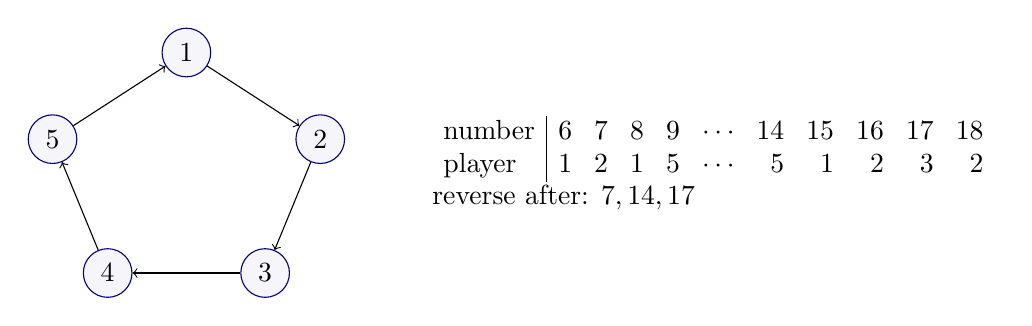
\begin{tikzpicture}[every node/.style={font=\normalsize},p/.style={circle,draw=NavyBlue,fill=NavyBlue!4,minimum size=.6cm}]
\node[p] (p1) at (0,1.4) {1};\node[p] (p2) at (1.7,.3) {2};\node[p] (p3) at (1,-1.4) {3};\node[p] (p4) at (-1,-1.4) {4};\node[p] (p5) at (-1.7,.3) {5};
\draw[->] (p1)--(p2);\draw[->] (p2)--(p3);\draw[->] (p3)--(p4);\draw[->] (p4)--(p5);\draw[->] (p5)--(p1);
\node[align=left,anchor=west] at (3,0) {\setlength{\tabcolsep}{4pt}\begin{tabular}{l|rrrrrrrrrr}
number&6&7&8&9&$\cdots$&14&15&16&17&18\\
player&1&2&1&5&$\cdots$&5&1&2&3&2
\end{tabular}\\reverse after: $7,14,17$};
\end{tikzpicture}
\figcap{The arrows show the initial clockwise order. The spoken number changes the next direction, not the player who has already spoken it. Player 2 says 18.}
\end{fig}
\begin{shortcuts}
\ii To convert a loop, name each changing quantity and make it a helper argument. Keep fixed inputs in the enclosing function. The stopping test and the state update remain the same.
\ii A \textbf{tail call} supplies the whole result directly, as in \py{return fact\_k(...)}. In ordinary factorial, multiplication still waits after the recursive return. Python retains call frames in both cases; tail recursion is not a constant-memory loop optimization here.
\end{shortcuts}
\begin{trapbox}
\ii In Twenty-One, the final mover loses; in Hog, reaching the goal wins. Returning the same player's index in both games reverses one game's result.
\ii In Sevens, reversing after changing \py{who} makes the first wrong transition at 7: the next speaker should be Player 1 for 8, not Player 3.
\end{trapbox}

\section{Use separate functions for separate remaining tasks}
\begin{qbox}
How can checking evenness turn into checking oddness on a smaller integer? When counting distinct prime factors of 72000, why should repeated factors 2 count only once?
\end{qbox}
Two functions are \textbf{mutually recursive} if each calls the other, possibly through a nested helper. Each still needs a precise contract, base cases and progress. For nonnegative integers,0 is even; a positive integer is even exactly when one less is odd:
\codeblock{parity}
\py{is\_even(4)} calls \py{is\_odd(3)}, \py{is\_even(2)}, \py{is\_odd(1)}, \py{is\_even(0)}, and returns true through those calls. Substituting the odd body gives an equivalent single function: if $n=0$, return true; if $n-1=0$, return false; otherwise return \py{is\_even(n-2)}. These tests avoid recursing to negative integers.
\method{Keep two game strategies separate --- CP 1.7.}
With $n$ pebbles, Alice always removes 1. Bob removes 2 when $n$ is even, otherwise 1. They alternate, Alice starts, and the final remover wins. At the beginning of a player's call, zero pebbles means the \emph{other} player just won:
\codeblock{alice_bob}
For 20, Alice leaves 19, Bob leaves 18, Alice leaves 17, and so on; Bob eventually removes the final pebble and the output is \py{Bob wins!}. Each actual turn decreases the positive remaining count. Only one recursive call runs per turn even though the function text has multiple branches.

\method{Remove one prime's entire multiplicity --- Lecture 10 slide 11 and 10.py.}
For $n>1$, let $k$ be its least divisor greater than 1. It is prime: if $k$ had a factor strictly between 1 and $k$, that smaller factor would also divide $n$, contradicting minimality. The helper \py{no\_k(n)} removes copies of this fixed $k$, then resumes counting the other distinct primes.
\codeblock{unique_factors}
\par\noindent\begin{minipage}{\linewidth}
\begin{steps}
\ii The divisor search eventually tests $n$, so it finds a divisor. Count its least prime $k$ once. Repeated division by $k$ decreases the remaining integer until it is 1 or is not divisible by $k$.
\ii At 1 there are no remaining factors; return 0. Otherwise the residual input is greater than 1 with no factor $k$, so a new distinct-prime count is required. Add that count to the one already counted.
\ii Integer prime factorization is unique (cited elementary number-theory fact). Therefore removing all copies of $k$ leaves exactly the other distinct prime factors, proving that none is lost or counted twice.
\end{steps}
\end{minipage}\par
For 72000=$2^6\cdot3^2\cdot5^3$, the residual inputs after each distinct factor are 72000 $\to$1125 $\to$125 $\to$1, giving 3. Genuine 10.py also checks 51=$3\cdot17$ gives 2;9=$3^2$ gives 1;576=$2^6\cdot3^2$ gives 2.
\begin{shortcuts}
\ii Give every helper a behavioral sentence: \py{no\_k} counts distinct primes other than its retained $k$; a primality-search helper tests whether any candidate divisor remains. The sentence determines its base result.
\ii A nested helper can read fixed $n$ or $k$ through its parent rather than receiving that same argument on every call. Lecture 9's \py{exp(x)} example makes this explicit:
\end{shortcuts}
\codeblock{exp_parent}
The call \py{exp(3)(2)} finds local $b=2$, enclosing $x=3$, then global \py{pow}, giving 8. In the lecture's repeated New Print example, the two new\_print frames likewise retain different print values. The five user calls are two wrapper constructions, the outer wrapper on 2, the first wrapper on 2, then the first wrapper on \py{'What?'}. Their final printed lines remain 2, What?, print returned What?, as derived in Week 3.
\begin{trapbox}
\ii The source's \py{unique\_prime\_factors} has contract $n>1$. Calling it on 1 enters a least-divisor search with no possible divisor greater than 1; its helper does not reach a base case. The internal \py{no\_k(1)} case is a different call and correctly returns 0.
\ii The functions' environments follow their recorded parents, not the call sequence. In \py{exp(3)(2)}, the base call's parent is the retained exp call; ordinary global recursion instead gives every recursive call Global as parent.
\end{trapbox}

\section{Place output before and after a recursive call}
\begin{qbox}
How can one call on 2013 print 2013,201,20,2 and then print 20,201,2013 on the return? Why is 2 printed only once?
\end{qbox}
\codeblock{cascade}
\par\noindent\begin{minipage}{\linewidth}
\begin{steps}
\ii Every call prints its current $n$ first. If it has at least two digits, it calls the function on $n//10$, then waits for that entire call to finish.
\ii The single-digit call prints 2 and makes no further call or trailing print. Returning to the call on 20 reaches its second print, then returning to 201 reaches that print, and finally 2013 prints again.
\ii Thus the exact output for 2013 is 2013,201,20,2,20,201,2013, one per line. Every call returns None; returning values and printing lines are separate actions.
\end{steps}
\end{minipage}\par
\begin{fig}
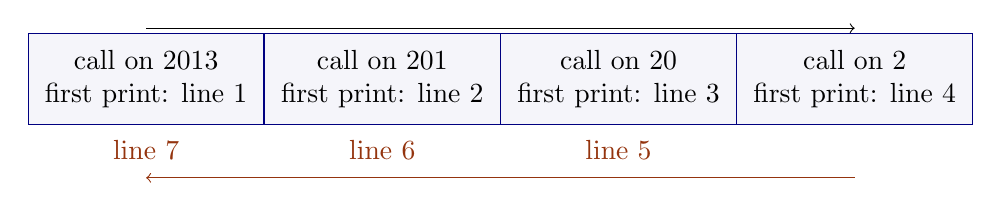
\begin{tikzpicture}[every node/.style={font=\normalsize}]
\foreach \x/\n/\a/\z in {0/2013/1/7,3/201/2/6,6/20/3/5,9/2/4/0}{
\node[draw=NavyBlue,fill=NavyBlue!4,align=center,inner sep=6pt] at (\x,0) {call on $\n$\\first print: line $\a$};
\ifnum\z>0 \node[RawSienna] at (\x,-.9) {line $\z$};\fi}
\draw[->] (0,.65)--(9,.65);\draw[->,RawSienna] (9,-1.25)--(0,-1.25);
\end{tikzpicture}
\figcap{The top arrow follows calls to shorter prefixes; the lower arrow follows their returns. The innermost one-digit call has no second print.}
\end{fig}
CP's longer equivalent form tests $n<10$ first and prints $n$ in that branch; its else branch prints $n$, recurses and prints $n$ again. Moving the print common to both branches before the test gives the displayed shorter form.
\begin{shortcuts}
\ii To trace output, write a line when its print executes. A line after the recursive call must wait until all lines of that smaller call have been written.
\ii Swipe uses the same arrangement but prints \py{n\%10} rather than the whole prefix. At 2837 it prints 7,3,8,2,8,3,7. The center remains a one-digit base case.
\end{shortcuts}
\begin{trapbox}
\ii Printing after every return would print the center digit twice. The second print belongs only to the branch that actually makes a recursive call.
\ii \py{return cascade(n//10)} would end the current call immediately after its subcall; a later print in that call would be unreachable.
\end{trapbox}

\section{Split possibilities into disjoint cases}
\begin{qbox}
How many ways can 6 be written as a sum of positive parts at most 4, ignoring order? What exact distinction lets two smaller counts be added without double counting?
\end{qbox}
A \textbf{tree-recursive} computation makes more than one recursive call in a single call's execution. For nonnegative integers, Fibonacci has $F_0=0$, $F_1=1$ and $F_n=F_{n-2}+F_{n-1}$ for $n\ge2$:
\codeblock{fib}
For $n=4$, the root calls fib(2) and fib(3); fib(3) calls fib(1) and fib(2) again. The two fib(2) calls each return 1, but they are distinct computations. This gives fib(4)=$1+2=3$ and fib(6)=8. The iterative two-value method avoids this repeated work; the recursive definition directly states which smaller results are combined.
\begin{fig}
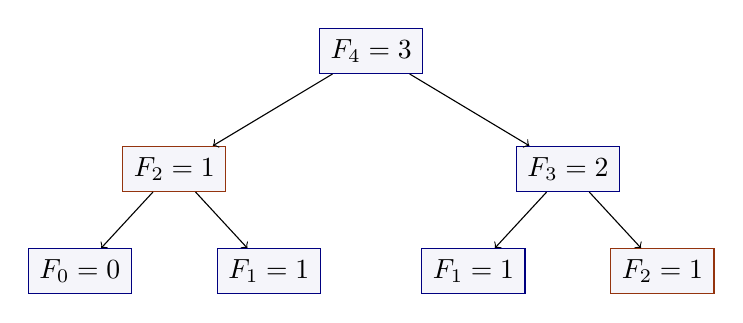
\begin{tikzpicture}[box/.style={draw=NavyBlue,fill=NavyBlue!4,inner sep=4pt}]
\node[box] (a) at (0,1.5) {$F_4=3$};
\node[box,draw=RawSienna] (b) at (-2.5,0) {$F_2=1$};
\node[box] (c) at (2.5,0) {$F_3=2$};
\node[box] (d) at (-3.7,-1.3) {$F_0=0$};
\node[box] (e) at (-1.3,-1.3) {$F_1=1$};
\node[box] (f) at (1.3,-1.3) {$F_1=1$};
\node[box,draw=RawSienna] (g) at (3.7,-1.3) {$F_2=1$};
\draw[->] (a)--(b);\draw[->] (a)--(c);
\draw[->] (b)--(d);\draw[->] (b)--(e);
\draw[->] (c)--(f);\draw[->] (c)--(g);
\end{tikzpicture}
\figcap{Actual calls for fib(4). The two highlighted fib(2) calls recompute the same result; the right one's identical smaller calls are omitted from this compact picture.}
\end{fig}


A \textbf{partition} of $n$ using parts at most $m$ is a nondecreasing sequence of positive integers with sum $n$. Repeated parts are allowed;2+4 and 4+2 describe the same partition, so list it only in nondecreasing order. A part 5 is invalid when $m=4$.
\begin{proposition*}[Include/exclude recurrence --- CP 1.7; Lecture 10 slides 13--15]
For integers $n>0,m>0$, the partition count satisfies
\[P(n,m)=P(n-m,m)+P(n,m-1).\]
The bases are $P(0,m)=1$ for $m\ge0$, $P(n,m)=0$ for $n<0$, and $P(n,0)=0$ for $n>0$.
\end{proposition*}
\begin{motive}
\ii[Want.] Count every partition exactly once.
\ii[First try.] Choosing the first part freely can count different orders of the same parts.
\ii[Key step.] Separate partitions that use an $m$ from partitions that use no $m$. Remove one $m$ in the first group; keep the bound $m$ because another $m$ may remain. Lower the bound to $m-1$ in the second group. The groups cannot overlap.
\end{motive}
\par\noindent\begin{minipage}{\linewidth}
\begin{steps}
\ii Removing one final $m$ from a partition containing $m$ leaves a partition of $n-m$ with parts at most $m$. Appending one $m$ reverses this operation, so the first group has size $P(n-m,m)$.
\ii A partition containing no $m$ uses only parts at most $m-1$, giving the second count. Each partition is in exactly one group, so adding gives the recurrence.
\ii Empty sum 0 has one partition, with no parts. A negative target is impossible; a positive target with no positive parts available is impossible. These facts give all bases. With nonnegative $m$, each recursive call decreases $n+m$ before a base is reached.
\end{steps}
\end{minipage}\par
\codeblock{partitions}
\begin{fig}
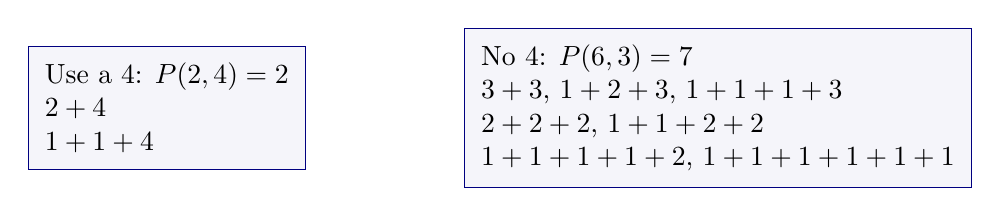
\begin{tikzpicture}[box/.style={draw=NavyBlue,fill=NavyBlue!4,align=left,inner sep=6pt}]
\node[box] (a) at (0,0) {Use a 4: $P(2,4)=2$\\$2+4$\\$1+1+4$};
\node[box] (b) at (7,0) {No 4: $P(6,3)=7$\\$3+3$, $1+2+3$, $1+1+1+3$\\$2+2+2$, $1+1+2+2$\\$1+1+1+1+2$, $1+1+1+1+1+1$};
\end{tikzpicture}
\figcap{All nine actual partitions of 6 with parts at most 4. Presence of a part equal to 4 separates the two groups; removing it leaves the smaller target 2.}
\end{fig}
The source's other counts are $P(5,5)=7$, $P(10,10)=42$, $P(15,15)=176$, and $P(20,20)=627$. The supplied code assumes $m\ge0$; its equality test $m=0$ does not cover arbitrary negative starting bounds.

\method{Use the same case distinction for other counts and maxima.}
HW3 Count Coins uses denominations 1,5,10,25. At a current denomination $c$, either use one $c$ and keep it available, or use none and move to the supplied next-smaller coin. One exact-change completion contributes 1; overshooting the target or exhausting denominations contributes 0. This is the same include/exclude argument with a different allowed-part list.

For HW3 Maximum Subsequence, split by whether the last digit is used. At most $t$ digits may be kept: using it leaves $t-1$ slots; skipping it leaves $t$ slots. Append a kept digit $d$ by multiplying the preceding numeric result by 10 and adding $d$. For 20125 with $t=3$, the two best candidates are $22\cdot10+5=225$ and 212, so the answer is 225. The branches take a maximum, rather than adding counts.

Lecture 10's \py{count\_park(n)} counts arrangements of $n$ adjacent spots: an empty spot \py{.} and a motorcycle \py{\%} each use one spot; a car \py{<>} uses two. Choose the first object: the two one-spot choices each leave $n-1$ spots, while a car leaves $n-2$:
\codeblock{parking}
For 1 spot, \py{.} and \py{\%} give 2. For 2 spots, \py{..}, \py{.\%}, \py{\%.}, \py{\%\%}, \py{<>} give 5. Then the recurrence gives counts 12 and 29 for 3 and 4 spots. An empty arrangement contributes 1 at $n=0$; a negative remaining length contributes 0.
\begin{shortcuts}
\ii Before adding two recursive counts, explain why their objects cannot overlap and why their union includes every object being counted. Before taking a maximum, identify which candidate each branch optimizes.
\ii Keep the current denomination after using it: another copy may be needed. Lowering it in both branches incorrectly forbids repeated coins.
\end{shortcuts}
\begin{trapbox}
\ii Returning 0 for target 0 discards a completed solution. In a sum of counts, success contributes 1 even though no parts remain to choose.
\ii Multiple recursive-looking lines in different if branches need not cause tree recursion. The Alice/Bob game executes only one of its recursive calls on each turn; Fibonacci executes both subcalls.
\end{trapbox}

\section{Test every digit, then test successive prefixes}
\begin{qbox}
What is the largest prefix of 94720 whose digits are all odd? How can a function that tests one digit be reused to test an entire candidate prefix?
\end{qbox}
This is Lecture 8's reproduction of Spring 2025 MT1 Q3(a--c). A digit predicate cond maps a digit 0--9 to a Boolean. A \textbf{prefix} of positive $n$ is $n//10^p$ for an integer $p\ge0$;3456 has prefixes 3456,345,34,3 and 0. The helper below tests every digit of a positive candidate:
\codeblock{all_digits}
Before each test all removed digits passed cond. One failure returns false; reaching zero without a failure returns true. With \py{odd=lambda d:d\%2==1},123 fails after testing 3 then 2;357 passes after testing 7,5,3.
\codeblock{prefix_process}
\par\noindent\begin{minipage}{\linewidth}
\begin{steps}
\ii Process tests the positive prefixes in decreasing order. Its check receives the whole candidate, so the supplied lambda calls all\_digits on that candidate with the retained cond.
\ii The first successful candidate is therefore the largest. If every positive prefix fails, return 0 as the source's no-positive-prefix result.
\ii For 94720 with odd,94720,9472,947 and 94 each contain an even digit;9 passes. For 919321 the first two candidates fail at 2 and 9193 passes. Source cases 2025/odd and 20252025/digit $<4$ give 0 and 202; an always-true test on 20252025 returns the entire number.
\end{steps}
\end{minipage}\par
\method{The supplied single-loop alternative --- Spring 2025 MT1 Q3(c).}
\codeblock{prefix_loop}
Before each test,$k$ counts the already-checked rightmost digits of the current $n$. When a digit passes, increase $k$; when one fails, shorten $n$ and restart checking at $k=0$. A positive $n<10^k$ means every digit of that current candidate has passed. This method tests some digits repeatedly but returns the same largest prefix for a stable digit predicate. The renamed suffix \py{\_loop} distinguishes the two original alternatives, both named prefix\_digits in the source.

\method{A zero-argument helper can read the current loop state --- Spring 2025 MT1 Q4.}
\codeblock{numbered_hailstone}
The source names this function hailstone; the descriptive prefix distinguishes it from Discussion 3's different output contract. At $n=10$, the exact lines are \py{1 10 -> 5}, \py{2 5 -> 16}, \py{3 16 -> 8}, \py{4 8 -> 4}, \py{5 4 -> 2}, \py{6 2 -> 1}. Its helper reads the current enclosing $n,k$, prints an update and returns the next $n$. Simultaneous assignment evaluates \py{k+1} and \py{f()} before rebinding either name, so the helper sees the old counter. This function returns None, whereas Discussion 3 returns the number of terms.
\begin{shortcuts}
\ii Lecture 8 also asks for square/cube without lambda or \py{**} in the answer. Reverse exchanges two arguments; curry supplies them one at a time:
\end{shortcuts}
\codeblock{reverse_curry}
\py{reverse(pow)(2,3)=pow(3,2)=9}; \py{curry(pow)(5)(2)=25}. The new square fixes the \emph{exponent} 2 before the base arrives; square(3) gives 9 and cube(3) gives 27. The unchanged lecture 08.py ends with an unfilled blank and cannot run as downloaded; the completed constructions above fill that actual exercise.
Lecture 8 slide 17 also rewrites the actual nested-lambda expression
\[\py{(lambda f: lambda x: f(f(x)))(lambda y: y*y)(3)}=81.\]
The inner applications give $3\to9\to81$. Replace each lambda by a fresh local definition with the same parameters, return expression and defining frame; this produces the source's equivalent twice/square definitions without changing this computation.
\begin{trapbox}
\ii \py{curry(pow)(2)} fixes the base 2, giving $2^x$ rather than $x^2$. Reverse is necessary to supply the exponent first.
\ii A digit predicate does not directly test a whole multi-digit prefix. Use a wrapper to test a whole prefix: \py{lambda k: all\_digits(k,cond)}. It adapts the input contract.
\end{trapbox}

\section{Problem set}
\subsection{Discussion 3 and related Lecture 10 practice}
\begin{prob}
\textbf{Q1: Swipe.} Print the digits of a positive integer $n$ backward and then forward, one per line, with the leftmost digit printed once. No \py{while}, \py{for}, or \py{str}. For 2837 the output is 7,3,8,2,8,3,7. The supplied base is \py{if n<10: print(n)}; fill its else branch.\par
\hint{Use the before/call/after arrangement from cascade, printing just the last digit.}
\end{prob}
\begin{prob}
\textbf{Q2: Skip Factorial.} For positive integer $n$, return $n(n-2)(n-4)\cdots$ down to 1 or 2. Fill the base condition, base return and recursive return. Source checks:5 gives 15;8 gives 384.\par
\hint{One base condition can include both possible final factors.}
\end{prob}
\begin{prob}
\textbf{Q3: Is Prime.} For integer $n>1$, implement a recursive primality test with no while/for. Source tests:2 true,16 false,521 true. Use a helper with as few arguments as possible, and give its docstring a precise behavioral description. The suggested template is:
\begin{lstlisting}
def is_prime(n):
    def f(i):
        if i == n:
            return __________
        elif ________________:
            return __________
        else:
            return f(________)
    return f(2)
\end{lstlisting}
\hint{Retain n in the outer frame; the helper searches candidate divisors from i through n-1.}
\end{prob}
\begin{prob}
\textbf{Q4: Recursive Hailstone.} For positive integer $n$, print every term through 1 and return the number of elements, including the first and last. For 10, output 10,5,16,8,4,2,1 and return 7; at 1 print 1 and return 1. Preserve the supplied split into hailstone/even/odd:
\begin{lstlisting}
def hailstone(n):
    print(n)
    if n % 2 == 0:
        return even(n)
    else:
        return odd(n)

def even(n):
    return __________________

def odd(n):
    # Complete this helper.
    _________________________
\end{lstlisting}
\hint{An even input always continues; an odd input has a special base at 1. Count the current term in each helper's returned value.}
\end{prob}
\begin{prob}
\textbf{Q5: Sevens.} Implement \py{sevens(n,k)} for positive integers $n,k$, returning which of the $k$ numbered players says $n$ under the direction rule developed above. The source requires helper \py{f(i,who,direction)}, with base \py{if i==n:return who} and initial call \py{f(1,1,1)}; supplied has\_seven removes digits recursively. Source inputs $n=2,6,7,8,9,18$, each with $k=5$, give 2,1,2,1,5,2.\par
\hint{Switch the direction at the current spoken number, advance/wrap who, then recurse on i+1.}
\end{prob}
\begin{prob}
\textbf{Spring 2024 MT1 Q4(e), reproduced in Lecture 10 slide 6: Streak.} A dice integer has every digit in 1--6. For positive $n$, return whether it is a dice integer with every digit the same. Fill the two source blanks:
\begin{lstlisting}
def streak(n):
    return (n >= 1 and n <= 6) or (
        n > 9 and _______________ and streak(________))
\end{lstlisting}
Source true cases 22222,4,33333333333333; false 22322,99999,505,707,7070.\par
\hint{A one-digit valid die is a base; a longer number needs equal last two digits and a valid shorter streak.}
\end{prob}
\begin{prob}
\textbf{Q6 (optional): Karel the Robot.} Karel starts at the bottom-left corner of an unknown $n\times n$ square. Use the east-facing start of the \href{https://compedu.stanford.edu/karel-reader/docs/python/en/ide.html}{linked default UI}. Four available functions: \py{move()} advances one square or errors at a wall; \py{turn\_left()} turns 90 degrees left; \py{front\_is\_blocked()} and \py{front\_is\_clear()} test the square ahead. End in the middle of the bottom row, in any orientation: for 7, column 4; for even $n$, either column $n//2$ or $n//2+1$.

Only if/if-else statements and function calls may appear in main's body. No assignment, nested def, lambda, while or for. You may call main recursively. The discussion prose omits the initial heading; the linked UI's bottom-left/east default supplies the orientation used here.\par
\hint{Advance two squares before the recursive call, then return one square while coming back. Specify the direction in which each smaller call finishes.}
\end{prob}

\subsection{Homework 3 --- due September 24 at 11:59p.m.}
\begin{prob}
\textbf{Q1: Num Eights.} For positive integer $n$, return its number of 8 digits using recursion. No assignment statements of any kind or loops, including in helpers. Source checks:3 $\mapsto$0,8 $\mapsto$1,88888888 $\mapsto$8,2638 $\mapsto$1,86380 $\mapsto$2,12345 $\mapsto$0,8782089 $\mapsto$3.\par
\hint{Separate the last digit's contribution from the count on the remaining prefix.}
\end{prob}
\begin{prob}
\textbf{Q2: Digit Distance.} Return the sum of absolute differences between consecutive digits of positive integer $n$. Use recursion and no loops. Source illustrations:61 gives 5;71253 gives $6+1+3+2=12$;6 gives 0. Starter tests:3 $\mapsto$0,777 $\mapsto$0,314 $\mapsto$5,31415926535 $\mapsto$32,3464660003 $\mapsto$16.\par
\hint{Removing the last digit removes exactly one adjacent pair.}
\end{prob}
\begin{prob}
\textbf{Q3: Interleaved Sum.} For positive integer $n$, compute $f_{\mathrm{odd}}(1)+f_{\mathrm{even}}(2)+f_{\mathrm{odd}}(3)+\cdots$ through $n$. Do not directly test parity. No loops, \py{\%}, \py{//}, multiplication, or bitwise \py{\& | \textasciicircum} in the function or its helpers; the public tests ban these syntax nodes individually. With identity, square and triple, source cases are $(5,\mathrm{identity},\mathrm{square})=29$, $(5,\mathrm{square},\mathrm{identity})=41$, $(4,\mathrm{triple},\mathrm{square})=32$, $(4,\mathrm{square},\mathrm{triple})=28$.\par
\hint{The first index is known to be odd; alternate two helpers whose names determine which function to apply.}
\end{prob}
\begin{prob}
\textbf{Q4: Count Coins.} Count unordered ways to make positive integer total using 1,5,10,25-cent coins. Use recursion, no loops, and the supplied next\_smaller\_coin:25 $\to$10 $\to$5 $\to$1 $\to$ None. At 15 there are six ways: fifteen 1s; ten 1s+one 5; five 1s+two 5s; five 1s+one 10; three 5s; one 5+one 10. Starter totals 15,10,20,45,100,200 give 6,4,9,39,242,1463.\par
\hint{Use the include/exclude recurrence at the current denomination; test for None before subtracting a coin value.}
\end{prob}
\begin{prob}
\textbf{Q5: Maximum Subsequence.} For a nonnegative integer $n$ and nonnegative integer limit $t$, return the largest numeric value obtainable by keeping at most $t$ digits in their original order. Use recursion, no loops. A subsequence need not be contiguous. Source checks: $(2012,2)\mapsto22$, $(20125,3)\mapsto225$, $(20125,5)$ and $(20125,6)$ both give 20125; $(12345,3)\mapsto345$, $(12345,0)\mapsto0$, $(12345,1)\mapsto5$. Numeric zero represents the empty choice as well as all-zero choices.\par
\hint{Either append the last digit to the best shorter subsequence with t-1 slots, or skip it and keep t slots.}
\end{prob}
\begin{prob}
\textbf{Q6 (just for fun, outside required course scope): Towers of Hanoi.} Move a stack of $n\ge1$ disks from rod start to a different rod end among 1,2,3. Initially all disks are on start; smaller disks are above larger ones and the other rods are empty. Move one top disk at a time, never onto a smaller disk. Use the given print\_move function to print each move, and retain the supplied valid-rod assertion. The starter also describes subproblems where larger disks remain under the stack being moved.\par
\hint{Move the top n-1 disks to the spare rod, move the largest disk, then move the n-1 disks to the destination.}
\end{prob}
\begin{prob}
\textbf{Q7 (just for fun, outside required course scope): Anonymous Factorial.} Return one expression computing a factorial function, using only calls, conditional expressions and lambdas. No assignment/def statements in the returned expression, and do not refer to make\_anonymous\_factorial. Supplied imports are sub and mul from operator. Source check: the returned function at 5 gives 120.\par
\hint{A parameter can give the recursive function a local name; pass that function itself as an argument.}
\end{prob}
\par\noindent\begin{minipage}{\linewidth}
Check with \py{python3 -m pytest -k num\_eights}, replacing the final name for each other function. Prepare the Provenance submission bundle in VS Code and upload its zip to Gradescope. The official assignment also requires a checkoff interview; the just-for-fun puzzles are explicitly outside required course scope. Hog continues from Week 2 and is due September 17; no new lab is assigned this week.
\end{minipage}\par

\subsection{Assigned real exam practice}
\begin{prob}
\textbf{Fall 2017 MT1 Q4(a): Digital, p5 (linked by HW3).} Implement collapse for a nonnegative integer $n$, removing any digit equal to the digit immediately to its right, so no adjacent digits agree. Source checks:1234 $\mapsto$1234;12234441 $\mapsto$12341;0 $\mapsto$0;3 $\mapsto$3;11200000013333 $\mapsto$12013. Fill the original template:
\begin{lstlisting}
def collapse(n):
    left, last = n // 10, n % 10
    if ______________________:
        return last
    elif ______ == __________:
        return collapse(_____)
    else:
        return collapse(_____) * 10 + _____
\end{lstlisting}
\hint{Compare the last two digits; either discard a duplicate or append a different last digit after collapsing the prefix.}
\end{prob}
\begin{prob}
\textbf{Fall 2019 Final Q6(b): Palindromes, p6 (linked by HW3).} Implement contains(a,b) to test whether the digits of nonnegative integer $a$ appear in order among the digits of nonnegative integer $b$. No \py{str, repr, list, tuple, [, ]}. Source checks: \py{contains(357,12345678)} true, \py{contains(753,12345678)} false, \py{contains(357,37)} false. Follow the official solution's convention that $a=0$ denotes no remaining digits, including an initial 0; it is not a requirement to find the written digit 0.
\begin{lstlisting}
def contains(a, b):
    if a == b:
        return True
    if ______ > ______:
        return False
    if ______ == ______:
        return contains(______, ______)
    else:
        return contains(______, ______)
\end{lstlisting}
\hint{Match the requested last digit to the rightmost available matching digit of b, or discard a nonmatching last digit of b.}
\end{prob}

\textbf{Attribution.} Official Fall 2026 CS 61A lectures/assignments; Composing Programs 3ed section 1.7, CC BY-NC-SA 4.0. Original assigned exams: \href{https://cs61a.org/resources/fa17/mt1/61a-fa17-mt1.pdf}{Fall 2017 Midterm 1} and \href{https://cs61a.org/resources/fa19/final/61a-fa19-final.pdf}{Fall 2019 Final}. Other exam reproductions are identified above.

\end{document}
